% 6739 TV version 11/20/19
% improved integral examples


\documentclass{beamer}

%\usepackage{beamerthemesplit}
%\usepackage[psamsfonts]{amsfonts}
%\usepackage{epsfig,graphicx,subfig,amsmath,amssymb,latexsym,stmaryrd,color,float}
\usepackage{epsfig,colordvi}
\usepackage{amsmath,amssymb,latexsym,stmaryrd}
\usepackage{float}
%\usepackage{algpseudocode}
%\usepackage{natbib}%[square,numbers]{natbib}
%\usepackage{threeparttable}
%\usepackage{multirow}
% Setup appearance:
\usepackage{multirow}

\setbeamertemplate{footline}[page number]
\usetheme{Raleigh}
%\usetheme{Antibes}
\usecolortheme{lily}
%\usetheme{Darmstadt}
%\usetheme{juanlespins}
%\usefonttheme[onlylarge]{structurebold}
\usefonttheme{professionalfonts}
\setbeamerfont*{frametitle}{size=\normalsize,series=\bfseries}
\setbeamertemplate{navigation symbols}{}


% Standard packages

\usepackage[english]{babel}
%\usepackage[latin2]{inputenc}
\usepackage{times}
\usepackage[T1]{fontenc}
\usepackage{textcomp}     % access \textquotesingle
%
% Setup TikZ
%
\usepackage{tikz}
\usetikzlibrary{arrows}
\tikzstyle{block}=[draw opacity=0.7,line width=1.4cm]

% the next line supposedly puts logo in bottom left
%\logo{\includegraphics[width=.1\textwidth]{buzz_hover}\hspace*{.88\paperwidth}}
% the next line puts logo in bottom right
\logo{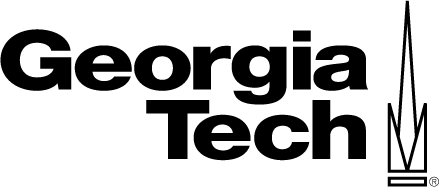
\includegraphics[width=.1\textwidth]{GT-Logo}}

\newcommand{\paws}{\pause}
\renewcommand{\paws}{}

\newcommand{\BC}{\begin{center}}
\newcommand{\EC}{\end{center}}
\newcommand{\BE}{\begin{equation}}
\newcommand{\EE}{\end{equation}}
\newcommand{\BEA}{\begin{eqnarray}}
\newcommand{\EEA}{\end{eqnarray}}
\newcommand{\BEAS}{\begin{eqnarray*}}
\newcommand{\EEAS}{\end{eqnarray*}}
\newcommand{\BEG}{\begin{example}\rm}
\newcommand{\EEG}{\end{example}}
\newcommand{\BTHM}{\begin{theorem}\rm}
\newcommand{\ETHM}{\end{theorem}}
\newcommand{\BCOR}{\begin{cor}\rm}
\newcommand{\ECOR}{\end{cor}}
\newcommand{\BPF}{\begin{proof}\rm}
\newcommand{\EPF}{\end{proof}}
\newcommand{\BRMK}{\begin{remark}\rm}
\newcommand{\ERMK}{\end{remark}}
\newcommand{\BLEM}{\begin{lemma}\rm}
\newcommand{\ELEM}{\end{lemma}}
\newcommand{\BIT}{\begin{itemize}}
\newcommand{\EIT}{\end{itemize}}
\newcommand{\DEF}{{\bfblue Definition}}
\newcommand{\RMK}{{\bfblue Remark}}
\newcommand{\RMKS}{{\bfblue Remarks}}
\newcommand{\THM}{{\bfblue Theorem}}
\newcommand{\COR}{{\bfblue Corollary}}
\newcommand{\PF}{{\bfblue Proof}}
\newcommand{\EG}{{\bfblue Example}}
\newcommand{\EGS}{{\bfblue Examples}}
\newcommand{\NOTN}{{\bfblue Notation}}


%\definecolor{myred}{HTML}{B3A369} % my tech gold from GT website
%\definecolor{myred}{HTML}{8E8B77} % Joe's tech gold
\definecolor{myred}{HTML}{EAAA00} % Joe's alternate gold
%\newcommand{\bfred}{\large \rm \color{myred}}
\newcommand{\bfred}{\bf \color{myred}}
%\newcommand{\bfred}{\color{red}}
%\definecolor{myblue}{HTML}{4277BB} % Joe's tech blue
\definecolor{myblue}{HTML}{003057} % Joe's alternate blue from GT website
%\newcommand{\bfblue}{\large \rm \color{myblue}}
\newcommand{\bfblue}{\bf \color{myblue}}
%\newcommand{\bfblue}{\color{blue}}
\newcommand{\myboldmath}{\boldmath} % turn this on if \bfred or \bfblue are actually using boldface (so that math symbol will also be in boldface}
%\newcommand{\myboldmath}{}

\newcommand{\dst}{\displaystyle}
\newcommand{\eq}{{\mbox{$\;\; = \;\;$}}}
\newcommand{\qbox}{{\mbox{\quad $\Box$}}}
\def\contradict
{
\tikz[baseline, x=0.2em, y=0.2em, line width=0.04em]
\draw (0,0) -- ({4*cos(45)},{4*sin(45)})
    (-1,1) -- ({-1 + 4*cos(45)},{1 + 4*sin(45)})
    (-1,3) -- ({-1 + 4*cos(315)},{3 + 4*sin(315)})
    (0,4) -- ({0 + 4*cos(315)},{4 + 4*sin(315)});
}
%
\newenvironment{proof2}[2][Proof of Theorem]{\textbf{#1 #2:} }{\hfill $\Box$} %{\ \ rule{0.5em}{0.5em}}
\newenvironment{proof3}[2][Proof of Theorems]{\textbf{#1 #2:} }{\hfill $\Box$} %{\ \ rule{0.5em}{0.5em}}
\newenvironment{assump}[1][Assumption]{\textbf{#1} }{\hfill $\Box$} %{\ \ rule{0.5em}{0.5em}}
%
\newcommand{\iid}{\mbox{$ \ \stackrel{\rm iid}{\sim} \ $}}
\newcommand{\bin}[2]{{{#1} \choose {#2}}}
\renewcommand{\Pr}{\mbox{$P$}} % Normal operator
\newcommand{\hs}[1]{\hspace{#1}}
\newcommand{\vs}[1]{\vspace{#1}}
\newcommand{\vsp}{\vspace{.1in}}
\newcommand{\ra}{\rightarrow}
\newcommand{\la}{\leftarrow}
\newcommand{\Ra}{\Rightarrow}
\newcommand{\RA}{\Longrightarrow}
\newcommand{\E}{\mathrm{E}} % expectation operator
\newcommand{\Var}{\mathrm{Var}} % Var operator
\newcommand{\Cov}{\mathrm{Cov}} % Cov operator
\newcommand{\Corr}{\mathrm{Corr}} % Corr operator
\newcommand{\Bias}{\mathrm{Bias}} % Bias operator
\newcommand{\MSE}{\mbox{MSE}} % MSE operator
\newcommand{\Nor}{\mbox{\rm Nor}} % Normal operator
\newcommand{\natlog}{\ell{\rm n}}
\newcommand{\bX}{\mbox{\bf X}}
\newcommand{\W}{\mathcal{W}} % stnd brown. motion operator
\newcommand{\B}{\mathcal{B}} % brown. bridge operator
\newcommand{\A}{\mathcal{A}}
\newcommand{\C}{\mathcal{C}}
\newcommand{\cid}{\mbox{$ \ \stackrel{d}{\longrightarrow} \ $}} % convergence in distribution
\newcommand{\ciD}{\mbox{$ \ \stackrel{\mathcal{D}}{\longrightarrow} \ $}} % convergence in distribution with D
\newcommand{\cip}{\mbox{$ \ \stackrel{p}{\longrightarrow} \ $}} % convergence in probability
\newcommand{\cas}{\mbox{$ \ \stackrel{a.s.}{\longrightarrow} \ $}} % almost sure (w.p. 1) convergence
\newcommand{\cm}{\mbox{$ \ \stackrel{L^1}{\longrightarrow} \ $}} % convergence in mean
\newcommand{\cqm}{\mbox{$ \ \stackrel{L^2}{\longrightarrow} \ $}} % convergence in quadradic mean
\newcommand{\zee}{\hbox{{\sf Z}\kern-.3550em\hbox{{\sf Z}}}} % set of natural numbers
\newcommand{\real}{\hbox{{I\kern-.1667em\hbox{R}}}} % set of real numbers
\newcommand{\BOX}{\rule[-2pt]{4pt}{8pt}}
\newcommand{\id}{\mathrm{d}} % d letter in integral
\renewcommand{\arraystretch}{1.25}
\definecolor{DB}{rgb}{0,0.08,0.45}
\definecolor{BB}{rgb}{0.1,0,0.35}
\definecolor{Bd}{rgb}{0.1,0,0.8}

\newcommand{\Simley}[1]{%
\begin{tikzpicture}[scale=0.11]
    \newcommand*{\SmileyRadius}{1.5}%
    \draw [fill=brown!10] (0,0) circle (\SmileyRadius)% outside circle
        %node [yshift=-0.22*\SmileyRadius cm] {\tiny #1}% uncomment this to see the smile factor
        ;

    \pgfmathsetmacro{\eyeX}{0.5*\SmileyRadius*cos(30)}
    \pgfmathsetmacro{\eyeY}{0.5*\SmileyRadius*sin(30)}
    \draw [fill=cyan,draw=none] (\eyeX,\eyeY) circle (0.15cm);
    \draw [fill=cyan,draw=none] (-\eyeX,\eyeY) circle (0.15cm);

    \pgfmathsetmacro{\xScale}{2*\eyeX/180}
    \pgfmathsetmacro{\yScale}{1.0*\eyeY}
    \draw[color=red, domain=-\eyeX:\eyeX]
        plot ({\x},{
            -0.1+#1*0.15 % shift the smiley as smile decreases
            -#1*1.75*\yScale*(sin((\x+\eyeX)/\xScale))-\eyeY});
\end{tikzpicture}%
}%

\newcommand{\SmallSimley}[1]{%
\begin{tikzpicture}[scale=0.11]
    \newcommand*{\SmileyRadius}{0.9}%
    \draw [fill=brown!10] (0,0) circle (\SmileyRadius)% outside circle
        %node [yshift=-0.22*\SmileyRadius cm] {\tiny #1}% uncomment this to see the smile factor
        ;

    \pgfmathsetmacro{\eyeX}{0.5*\SmileyRadius*cos(30)}
    \pgfmathsetmacro{\eyeY}{0.5*\SmileyRadius*sin(30)}
    \draw [fill=cyan,draw=none] (\eyeX,\eyeY) circle (0.15cm);
    \draw [fill=cyan,draw=none] (-\eyeX,\eyeY) circle (0.15cm);

    \pgfmathsetmacro{\xScale}{2*\eyeX/180}
    \pgfmathsetmacro{\yScale}{1.0*\eyeY}
    \draw[color=red, domain=-\eyeX:\eyeX]
        plot ({\x},{
            -0.1+#1*0.15 % shift the smiley as smile decreases
            -#1*1.75*\yScale*(sin((\x+\eyeX)/\xScale))-\eyeY});
\end{tikzpicture}%
}%

\def\double{\par\baselineskip=24pt}
\def\single{\par\baselineskip=12pt}
\def\oneandahalf{\par\baselineskip=18pt}

%\transboxin<1>
%\transglitter<2>
%\transwipe%<3>
%\transdissolve

\newcounter{lesson} 
% Copyright 2004 by Madhusudan Singh <madhusudan.singh@gmail.com>
%
% This file may be distributed and/or modified
%
% 1. under the LaTeX Project Public License and/or
% 2. under the GNU Public License.
%
% See the file doc/licenses/LICENSE for more details.

\ProvidesPackageRCS $Header: /cvsroot/latex-beamer/latex-beamer/themes/color/beamercolorthemebeaver.sty,v 1.2 2007/01/28 20:48:24 tantau Exp $


\mode<presentation>

\definecolor{brightred}{rgb}{1.0,0,0}
\definecolor{lightblue}{rgb}{0,0,1}
\definecolor{brightblue}{rgb}{0,0,1}
\definecolor{myblue}{HTML}{003057} 

\setbeamercolor{section in toc}{fg=black,bg=white}
%\setbeamercolor{alerted text}{fg=brightblue!99!gray}
\setbeamercolor{alerted text}{fg=myblue!99!gray}
\setbeamercolor*{palette primary}{fg=myblue!65!white,bg=gray!30!white}
\setbeamercolor*{palette secondary}{fg=myblue!65!white,bg=gray!15!white}
\setbeamercolor*{palette tertiary}{bg=myblue!65!white,fg=gray!10!white}
\setbeamercolor*{palette quaternary}{fg=myblue,bg=gray!5!white}

\setbeamercolor*{sidebar}{fg=brightred,bg=gray!15!white}

\setbeamercolor*{palette sidebar primary}{fg=brightred!10!black}
\setbeamercolor*{palette sidebar secondary}{fg=white}
\setbeamercolor*{palette sidebar tertiary}{fg=brightred!50!black}
\setbeamercolor*{palette sidebar quaternary}{fg=gray!10!white}

%\setbeamercolor*{titlelike}{parent=palette primary}
\setbeamercolor{titlelike}{parent=pallette primary,fg=myblue!65!white}
\setbeamercolor{frametitle}{bg=gray!10!white}
\setbeamercolor{frametitle right}{bg=gray!10!white}

\setbeamercolor*{separation line}{}
\setbeamercolor*{fine separation line}{}

\mode
<all>

% Copyright 2007 by Till Tantau
%
% This file may be distributed and/or modified
%
% 1. under the LaTeX Project Public License and/or
% 2. under the GNU Public License.
%
% See the file doc/licenses/LICENSE for more details.

\ProvidesPackageRCS $Header: /cvsroot/latex-beamer/latex-beamer/themes/inner/beamerinnerthemerounded.sty,v 1.5 2007/01/28 20:48:30 tantau Exp $


\DeclareOptionBeamer{shadow}[true]{\def\beamer@themerounded@shadow{#1}}
\ExecuteOptionsBeamer{shadow=false}
\ProcessOptionsBeamer

\mode<presentation>

\setbeamertemplate{blocks}[rounded][shadow=\beamer@themerounded@shadow]
\setbeamertemplate{items}[ball]
\setbeamertemplate{sections/subsections in toc}[ball]
\setbeamertemplate{title page}[default][colsep=-4bp,rounded=true,shadow=\beamer@themerounded@shadow]
\setbeamertemplate{part page}[default][colsep=-4bp,rounded=true,shadow=\beamer@themerounded@shadow]
  
\mode<all>

%%% Local Variables: 
%%% TeX-master: "~/texmf/tex/latex/beamer/test/test.tex"
%%% End: 

% Copyright 2007 by Till Tantau
%
% This file may be distributed and/or modified
%
% 1. under the LaTeX Project Public License and/or
% 2. under the GNU Public License.
%
% See the file doc/licenses/LICENSE for more details.

\ProvidesPackageRCS $Header: /cvsroot/latex-beamer/latex-beamer/themes/outer/beamerouterthemeinfolines.sty,v 1.9 2007/01/28 20:48:30 tantau Exp $


\mode<presentation>

\setbeamercolor*{author in head/foot}{parent=palette tertiary}
\setbeamercolor*{title in head/foot}{parent=palette secondary}
\setbeamercolor*{date in head/foot}{parent=palette primary}

\setbeamercolor*{section in head/foot}{parent=palette tertiary}
\setbeamercolor*{subsection in head/foot}{parent=palette primary}

\defbeamertemplate*{footline}{infolines theme}
{
  \leavevmode%
   \hbox{%
   \begin{beamercolorbox}[wd=.20\paperwidth,ht=2.25ex,dp=1ex,center]{author in head/foot}%
       \usebeamerfont{author in head/foot}\insertshortauthor
   \end{beamercolorbox}%
%\begin{beamercolorbox}[wd=.80\paperwidth,ht=2.25ex,dp=1ex,center]{title in head/foot}%
  \begin{beamercolorbox}[wd=.60\paperwidth,ht=2.25ex,dp=1ex,center]{title in head/foot}%
     \usebeamerfont{title in head/foot}%\insertshorttitle % make wd = .80 (80%) to kill off pg numering
   \end{beamercolorbox}%
  \begin{beamercolorbox}[wd=.20\paperwidth,ht=2.25ex,dp=1ex,right]{date in head/foot}%
    \usebeamerfont{date in head/foot}\insertshortdate{}\hspace*{2em}
    \insertframenumber{} / \inserttotalframenumber\hspace*{2ex} 
  \end{beamercolorbox}}%
  \vskip0pt%
}

\defbeamertemplate*{headline}{infolines theme}
{
  \leavevmode%
  \hbox{%
 % \begin{beamercolorbox}[wd=.5\paperwidth,ht=2.25ex,dp=1ex,right]{section in head/foot}%
  \begin{beamercolorbox}[wd=.5\paperwidth,ht=2.25ex,dp=1ex,left]{section in head/foot}%
    \usebeamerfont{section in head/foot}\hspace*{3.5ex}\insertsectionhead\hspace*{2ex}
  \end{beamercolorbox}%
  \begin{beamercolorbox}[wd=.5\paperwidth,ht=2.25ex,dp=1ex,left]{subsection in head/foot}%
    \usebeamerfont{subsection in head/foot}\hspace*{2ex}\insertsubsectionhead
  \end{beamercolorbox}}%
  \vskip0pt%
}

\setbeamersize{text margin left=1em,text margin right=1em}

\mode
<all>

% % Copyright 2004 by Madhusudan Singh <madhusudan.singh@gmail.com>
%
% This file may be distributed and/or modified
%
% 1. under the LaTeX Project Public License and/or
% 2. under the GNU Public License.
%
% See the file doc/licenses/LICENSE for more details.

\ProvidesPackageRCS $Header: /cvsroot/latex-beamer/latex-beamer/themes/theme/beamerthemeCambridgeUS.sty,v 1.2 2007/01/28 20:48:30 tantau Exp $


\mode<presentation>

\useinnertheme[shadow=true]{rounded}
\useoutertheme{infolines}
\usecolortheme{beaver}

\setbeamerfont{block title}{size={}}
\setbeamercolor{titlelike}{parent=structure,bg=white}
\mode
<all>


\date{1/15/20}
%\date{}

\title[]{\bfblue 0. Course Introduction + Bootcamps}
%\author[ISYE 6739]{\large Dave Goldsman} % Enter your name between curly braces
\author[ISYE 6739 --- Goldsman]{\large Dave Goldsman} % TURN ON FOR NON-TV NOTES
\institute[David Goldsman]{Georgia Tech} % Enter your institute name between curly braces
\institute[\ ]{H. Milton Stewart School of Industrial and Systems Engineering \\
Georgia Institute of Technology}

% CUSTOM DEFAULT BULLET FOR LISTS
\setbeamertemplate{itemize item}{\textbullet}
\setbeamercolor{itemize item}{fg=gray}
\setbeamercolor{itemize subitem}{fg=gray}
\setbeamercolor{enumerate item}{fg=gray}
\setbeamercolor{enumerate subitem}{fg=gray}

\setbeamertemplate{enumerate item}{\insertenumlabel.}

% CHANGE DEFAULT ITEM "LIST IMAGE"
\setbeamertemplate{itemize item}{\textbullet}
\setbeamercolor{itemize item}{fg=gray}
\setbeamercolor{enumerate item}{fg=gray}

\begin{document}

\rm

\begin{frame}
  \titlepage
\end{frame}

\begin{frame}\rm \frametitle{\bfblue Outline of Lessons}
  \tableofcontents
\end{frame}


%%%%%%%%%%%%%%%%%%%%%%%%%%%%%%

\section{Syllabus}
\label{sec:0.syllabus}
\AtBeginSection[]
{
   \begin{frame} \rm \frametitle{\bfblue Outline of Lessons}
       \tableofcontents[currentsection]
   \end{frame}
}

% \begin{frame}{\bfblue Lesson 0.\ref{sec:0.syllabus} --- Syllabus} \rm

% \paws

% \BC
% {\large \bfblue ISYE 6739 --- Probability and Statistics}
% \EC

% \paws

% {\bfblue Instructor}: Dave Goldsman \\
% %email: {\tt sman@gatech.edu} \\
% webpage: {\tt www.isye.gatech.edu/{\textasciitilde}sman} \\[12pt] \paws

% %{\bfblue Course Website}: {\tt canvas.gatech.edu}
% %\\[12pt] \paws

% {\bfblue Course Objectives}: Provide introduction to probability and statistics, emphasizing applications in science and engineering. \\[12pt] \paws

% {\bfblue Prerequisites}: You should be familiar with a spreadsheet package like Excel.  You should also know enough calculus
% to be able to integrate any easy function.  But if not, don't panic --- we'll have bootcamps for you!

% \end{frame}


% %\begin{frame} \rm
% %
% %{\bfblue Suggested Resources}: \paws
% %\BIT
% %\item Complete course notes (available on Canvas). \paws
% %\item {\bfred Free} pdf version of textbook! \paws
% %\item Helpful, happy teaching assistants! Office Hours!  Review Sessions! Quick Canvas responses! \paws
% %\item Grumpy old professor! Canvas stalking!
% %\EIT
% %
% %\paws
% %\vsp
% %
% %{\bfblue Grading}:
% %\BIT
% %\item Test 1 (30\%)
% %\item Test 2 (30\%)
% %\item Test 3 (30\%)
% %\item HW + if I like you (10\%)
% %\EIT
% %
% %\paws
% %\vsp
% %
% %{\bfblue Programming:} You'll be expected to do some elementary data analysis using your choice of packages such as Excel, R, etc.
% %
% %\end{frame}
% %
% %\begin{frame}
% %{\bfblue Course Format} \paws
% %\BIT
% %\item 8 {\bfred Modules} (including bootcamps)\ldots \paws
% %\item \ldots\ divided into about 100 {\bfred Lessons} (some are optional). \paws
% %\item Easy {\bfred Assessments} after each lesson. \paws
% %\item {\bfred Homework} each week. \paws
% %\BIT
% %\item You can discuss HW with friends, but the content is your responsibility. \paws
% %\item TAs and Canvas are very helpful. \paws
% %\item Plenty of Extra Credit opportunities --- can get HW grade $>$ 100\%!
% %\EIT
% %\paws
% %\item 3 {\bfred Tests} \paws
% %\BIT
% %\item Each test will be mostly based on the stuff since the last test, though anything up to that point is fair game. \paws
% %\item You'll be allowed $x$ two-sided standard-size (e.g., 8.5x11") cheat sheets for test $x$, where $x=1,2,3$. \paws
% %\item You'll be allowed to use a reasonable calculator. \paws
% %\item We'll supply all necessary tables. \paws
% %\item Plenty of practice tests will be available for you to study from.
% %\EIT
% %\EIT
% %
% %\end{frame}

% \begin{frame} \rm

% {\bfblue Syllabus} \paws
% \begin{enumerate}
% \setcounter{enumi}{-1}
% \item Set Theory and Calculus Bootcamps \paws
% \item Getting Started with Probability \paws
% \item Random Variables \paws
% \item Bivariate Random Variables \paws
% \item Distributions \paws
% \item Getting Started with Statistics \paws
% \item Confidence Intervals \paws
% \item Hypothesis Testing \paws
% \item Other Goodies (time permitting)
% \end{enumerate}

% \end{frame}

% %%%%%%%%%%%%%%%%%%%%%%%%%%%%%%

% \section{Introduction to Probability and Statistics}
% \label{sec:0.intro-prob}
% \AtBeginSection[]
% {
%   \begin{frame} \rm \frametitle{\bfblue Outline of Lessons}
%       \tableofcontents[currentsection]
%   \end{frame}
% }

% \begin{frame}{\bfblue Lesson 0.\ref{sec:0.intro-prob} --- Introduction to Probability and Statistics} \rm

% \paws

% {\bfblue Next Few Lessons:}
% \BIT
% \item This Probability and Statistics Intro
% \item Set Theory Bootcamp
% \item Calculus Bootcamps
% \EIT

% \vsp
% \paws

% Mathematical Models for describing observable phenomena:
% \BIT
% \item Deterministic
% \item Probabilistic
% \EIT

% \vsp
% \paws

% Deterministic Models
% \BIT
% \item Ohm's Law ($I=E/R$) (There's no place like Ohm.)
% \item Drop an object from height $h_0$.  After $t$ seconds, height $h(t) = h_0 - 16t^2$.
% \item Deposit \$1000 in a checking account, continuously compounding at 3\%. At time
% $t$, it's worth \$1000$e^{0.03t}$.
% \EIT


% \end{frame}

% \begin{frame} \rm

% %\transwipe

% {\bfred Probabilistic Models} --- Involve uncertainty \paws

% \BIT
% \item How much snow will fall tomorrow? \paws
% \item Will IBM make a profit this year?  \paws
% \item Should I buy a call or put option?  \paws
% \item Can I win in blackjack if I use a certain strategy?  \paws
% \item What is the cost-effectiveness of a new drug?  \paws
% \item Which horse will win the Kentucky Derby?
% \EIT

% \end{frame}

% \begin{frame} \rm

% {\bfblue Some Cool Examples} \\[12pt]   \paws

% \begin{itemize}
% \item Birthday Problem --- Assume all 365 days have equal probability of being a person's birthday
% (ignore freaks born on Feb.\ 29).  Then\ldots \\[12pt] \paws

% If there are {\bfred 23} students in a class, the odds are better than 50--50 that there will
% be a match. \\[12pt] \paws

% If there are {\bfred 50} students, the probability is about 97\%! \\[12pt] \paws

% \item Monopoly --- In the long run, the property having the highest probability of being
% landed on is Illinois Ave. \\[12pt] \paws

% \item Stock Market --- Monkeys randomly selecting stocks could have outperformed most market
% analysts during the past year.

% \end{itemize}
% \end{frame}

% \begin{frame} \rm

% \begin{itemize}
% \item
% Poker --- Pick 5 cards from a standard deck. Then \\[12pt] \paws
% \begin{itemize}
% \item[] $\Pr(\mbox{exactly 2 pairs}) \approx 0.0475$, \\[12pt]
% \item[] $\Pr(\mbox{full house}) \approx 0.00144$, \\[12pt]
% \item[] $\Pr(\mbox{flush}) \approx 0.00198$. \\[12pt]
% \end{itemize}

% \paws

% \item A couple has two kids and at least one is a boy. What's the probability
% that BOTH are boys? \\[6pt] \paws

% Possibilities:  GG, BG, GB, BB\@.  Eliminate GG since we know that there's at least
% one boy.  Then $\Pr(\mbox{BB}) = 1/3$. \\[12pt] \paws

% \item Ask Marilyn.  You are a contestant at a game show.
% Behind one of three doors is a car; behind the other two are goats.
% You pick door A\@. Monty Hall opens door B and reveals a goat.  Monty
% offers you a chance to switch to door C\@.  What should you do?  \paws Answer: SWITCH!

% \end{itemize}

% \end{frame}

% \begin{frame} \rm

% \begin{itemize}
% \item Vietnam Draft Lottery --- not as ``fair'' as you might think!\\[12pt] \paws

% \item Which is the most popular soft drink?  Well, in Atlanta, we know the answer to that one!  \\[12pt] \paws

% \item Why are some election polls so incredibly wrong? \\[12pt] \paws

% \item How do they do real-time updates of win probabilities as a basketball game progresses? \\[12pt] \paws

% \item How can you simulate randomness on a computer, and what can you use it for? \\[12pt] \paws

% \item How can you tell if the quality of an item that your manufacturing plant is producing has started to get worse?

% \end{itemize}
% \end{frame}


% \begin{frame} \rm

% {\bfblue Working Definitions} \\[12pt] \paws

% {\bfred Probability} --- Methodology that describes the random variation in systems.
% (We'll spend about 50\% of our time on this.) \\[12pt] \paws

% {\bfred Statistics} --- Uses sample data to draw general conclusions about the population
% from which the sample was taken.  (50\% of our time.)

% \end{frame}

% %%%%%%%%%%%%%%%%%%%%%%%%

% \section{The Joy of Sets Bootcamp}
% \label{sec:0.sets}
% \AtBeginSection[]
% {
%   \begin{frame} \rm \frametitle{\bfblue Outline of Lessons}
%       \tableofcontents[currentsection]
%   \end{frame}
% }

% %%%%%%%%%%%%%%%%%%%%%%%%%%%%%%%%%%%%%%%%%%%%%

% \begin{frame}{\bfblue Lesson 0.\ref{sec:0.sets} --- The Joy of Sets Bootcamp} \rm

% \paws

% {\bfblue Definition:} A {\bfred set} is a collection of objects.  Members of a set are called
% {\bfred elements}. \\[12pt] \paws


% {\bfblue Notation:} \paws \\[6pt]

% $A,B,C,\ldots$ for sets \paws \\[6pt]
% $a,b,c,\ldots$ for elements \paws \\[6pt]
% $\in$ for membership, e.g., $x \in A$ \paws \\[6pt]
% $\notin$ for non-membership, e.g., $x \notin A$ \paws \\[6pt]
% $U$ is the {\bfred universal set} (i.e., everything) \paws \\[6pt]
% $\emptyset$ is the {\bfred empty set}.

% \end{frame}

% \begin{frame} \rm

% {\bfblue Examples:} \\[12pt] \paws

% $A = \{1,2,\ldots,10\}$. $2 \in A$; $49 \notin A$. \\[12pt] \paws

% $B = \{\mbox{basketball, baseball}\}$ \\[12pt] \paws

% $C = \{x \,|\, 0 \le x \le 1 \}$  (``$\,|\,$'' means ``such that'') \\[12pt] \paws

% $D = \{x \,|\, x^2 = 9\} = \{\pm 3\}$ (either is fine) \\[12pt] \paws

% $E = \{x \,|\, x \in \mathbb{R}, x^2 = -1\} = \emptyset$ ($\mathbb{R}$ is the real line)

% \end{frame}

% \begin{frame} \rm

% {\bfblue Definition:} If every element of set $A$ is an element of set $B$
% then $A$ is a {\bfred subset} of $B$, i.e., $A \subseteq B$. \\[12pt] \paws

% {\bfblue Definition:} $A = B$ iff (if and only if) $A \subseteq B$ and $B \subseteq A$. \\[12pt] \paws

% {\bfblue Properties:} \\
% $\emptyset \subseteq A$; $A \subseteq U$; $A \subseteq A$ \\
% ($A \subseteq  B$  and $B \subseteq  C$) $\Ra$ (implies) $A \subseteq  C$ \\[12pt] \paws

% {\bfblue Remark:} The order in which the elements of a set are listed is immaterial, e.g., $\{a,b,c\} = \{b,c,a\}$.

% \end{frame}

% \begin{frame} \rm

% {\bfblue Definitions:} The  {\bfred complement} of $A$ with respect to $U$ is $\bar{A} \equiv
% \{x \,|\, x \in U \mbox{ and } x \notin A \}$. \\[12pt] \paws

% \RMK: Don't confuse complement with compliment! (``You are one fine-lookin' set!'') \\[12pt] \paws

% The {\bfred intersection} of $A$ and $B$ is $A \cap B \equiv
% \{x \,|\, x \in A \mbox{ and } x \in B \}$. \\[12pt] \paws

% The {\bfred union} of $A$ and $B$ is $A \cup B \equiv
% \{x \,|\, x \in A \mbox{ or } x \in B \mbox{ (or both)}\}$. \\[12pt] \paws

% (Remember {\bfred Venn diagrams}?)

% \end{frame}

% \begin{frame} \rm

% {\bfblue Example:} \\

% Suppose $U = \{\mbox{letters of the alphabet}\}$, $A = \{\mbox{vowels}\}^\star$,
% and $B=\{a,b,c\}$.  \\[6pt]

% $^\star${\footnotesize We'll ignore the fact that $y$ and $w$ are sometimes vowels  (believe it or not)!} \\[6pt] \paws


% Then \\[6pt]

% $\bar{A} = \{\mbox{consonants}\}$ \\
% $A \cap B = \{a\}$ \\
% $A \cup B = \{a,b,c,e,i,o,u\}.$ \qbox \\[12pt] \paws

% \DEF: If $A \cap B = \emptyset$, then $A$ and $B$ are {\bfred disjoint} (or {\bfred mutually
% exclusive}).

% \end{frame}

% \begin{frame} \rm

% {\bfblue More Definitions:} \\[12pt]

% {\bfred Minus}: $A - B \equiv A \cap \bar{B}$ \\[12pt] \paws

% \begin{center}
% 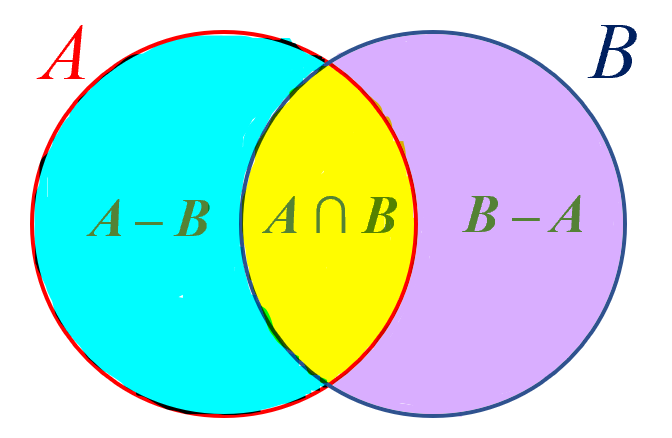
\epsfig{file=Module01-IntersectMinus.PNG,width=1.2in}
% \end{center}

% \paws

% {\bfred Symmetric difference} or {\bfred XOR}:
% \[
% A \, \Delta \, B \; \equiv \; (A-B) \cup (B-A)
% % = (A \cap \bar{B}) \cup (B \cap \bar{A}) \\
% \; = \; (A \cup B) - (A \cap B)
% \]

% \vs{.1in}

% \end{frame}

% \begin{frame} \rm

% The {\bfred cardinality} of $A$, denoted by $|A|$, is the number of elements in $A$.
% $A$ is {\bfred finite} if $|A| < \infty$.  \\[12pt] \paws


% {\bfblue Examples:} \\[6pt] \paws

% $A = \{3,4\}$ is finite, since $|A| = 2$. \\[12pt] \paws

% $B = \{1,2,3,\ldots\}$ is {\bfred countably infinite}, i.e., $|B| = \aleph_0$ (look up this symbol)! \\[12pt] \paws

% $C = \{x \,|\, x \in [0,1] \}$ is {\bfred uncountably infinite}, i.e., $|C| = \aleph_1$ (look it up)! \\[12pt]

% \end{frame}

% \begin{frame} \rm

% {\bfblue Laws of Operation:} \\[12pt] \paws

% \begin{itemize}

% \item[1.] {\bfred Complement Law:} $A \cup \bar{A} = U$, $A \cap \bar{A} = \emptyset$, $\bar{\bar{A}} = A$ \\[12pt] \paws

% \item[2.] {\bfred Commutative:} $A \cup B = B \cup A$, $A \cap B = B \cap A$ \\[12pt] \paws

% \item[3.] {\bfred Associative:} $A \cup (B \cup C) = (A \cup B) \cup C$, \\
% $A \cap (B \cap C) = (A \cap B) \cap C$ \\[12pt] \paws

% \item[4.] {\bfred Distributive:} $A \cup (B \cap C) = (A \cup B) \cap (A \cup C)$, \\
% $A \cap (B \cup C) = (A \cap B) \cup (A \cap C)$ \\[12pt] \paws

% \item[5.] {\bfred DeMorgan's:} $\overline{A \cup B} = \bar{A} \cap \bar{B}$,
% $\overline{A \cap B} = \bar{A} \cup \bar{B}$ \\[12pt] \paws

% \end{itemize}

% {\bfblue Proofs:}  Easy.  Could use Venn diagrams or many other ways.

% \end{frame}

% %%%%%%%%%%%%%%%%%%%%%%%%%%%%%%

% \section{Calculus Bootcamp: Introduction + Derivatives}
% \label{sec:0.calc-derivs}
% \AtBeginSection[]
% {
%   \begin{frame} \rm \frametitle{\bfblue Outline of Lessons}
%       \tableofcontents[currentsection]
%   \end{frame}
% }


% \begin{frame}{\bfblue Lesson 0.\ref{sec:0.calc-derivs} --- Calculus Bootcamp: Introduction + Derivatives} \rm

% %{\bfblue Goal:} This section provides a brief review of various calculus tidbits that we'll be using later on.  You can skip it if you feel so inclined. \\[12pt] \paws

% \paws

% \DEF: The {\bfred function} $f(x)$ maps values of $x$ from a certain {\bfred domain} $X$ to a certain {\bfred range} $Y$, which we can denote by the shorthand $f:X \rightarrow Y$.  \\[12pt] \paws

% \EG: If $f(x) = x^2$, then the function takes $x$-values from the real line $\mathbb{R}$ to the nonnegative portion of the real line $\mathbb{R}^{+}$. \\[12pt] \paws



% \DEF:  We say that $f(x)$ is a {\bfred continuous} function if, for any $x_0$ and $x \in X$, we have $\lim_{x\ra x_0} f(x) = f(x_0)$, where ``lim'' denotes a {\bfred limit} and $f(x)$ is assumed to exist for all $x \in X$. \\[12pt] \paws

% \EG: The function $f(x) = 3x^2$ is continuous for all $x$.  The function $f(x) = \lfloor x \rfloor$ (round down to the nearest integer, e.g., $\lfloor 3.4 \rfloor = 3$) has a ``jump'' discontinuity at any integer $x$. \quad $\Box$ \\[12pt]


% \end{frame}


% \begin{frame} \rm


% \DEF: The {\bfred inverse} of a function $f:X \rightarrow Y$ is (informally) the ``reverse'' mapping $g:Y \rightarrow X$ such that $f(x) = y$ if and only if $g(y) = x$ for all appropriate $x$ and $y$.  The inverse of $f$ is often written as $f^{-1}$, and is especially useful if $f(x)$ is a strictly increasing or strictly decreasing function. Note that $f^{-1}(f(x)) = x$. \\[12pt] \paws

% \EGS: If $f(x) = x^3$, then we have $f^{-1}(y) = y^{1/3}$.  If $h(x) = e^x$, then $h^{-1}(y) = \natlog(y)$. \qbox \\[12pt] \paws


% \DEF: If $f(x)$ is continuous, then it is {\bfred differentiable} (has a {\bfred derivative}) if
% \[
% \frac{d}{dx} f(x) \; \equiv \;  f'(x) \; \equiv \; \lim_{h\ra 0} \frac{f(x+h)-f(x)}{h}
% \]
% exists and is well-defined for any given $x$. Think of the derivative as the slope of the function. \\
% \end{frame}

% \begin{frame} \rm

% \EGS: Some well-known derivatives are: \paws
% \[
% [x^k]' \; = \; k x^{k-1},
% \]

% \paws

% \[
% [c^x]' \; = \; c^x \, \natlog(c), \; \; \mbox{and so} \; \; [e^x]' \; = \; e^x \; \; \mbox{(since $\natlog(e) = 1$)},
% \]

% \paws

% \[
% [\sin(x)]' \; = \; \cos(x),
% \]

% \paws

% \[
% [\cos(x)]' \; = \; -\sin(x),
% \]

% \paws

% \[
% [\natlog(x)]' \; = \; \frac{1}{x},
% \]

% \paws

% \[
% [\arctan(x)]' \; = \; \frac{1}{1+x^2}. \quad \Box
% \]

% \end{frame}

% \begin{frame} \rm

% \THM: Some well-known properties of derivatives are: \paws
% \[
% [a f(x) + b ]' \; = \; af'(x),
% \]

% \paws

% \[
% [f(x) + g(x)]' \; = \; f'(x) + g'(x),
% \]

% \paws

% \[
% [f(x)g(x)]' \; = \; f'(x)g(x) + f(x)g'(x) \quad \mbox{(product rule)},
% \]

% \paws

% \[
% \left[\frac{f(x)}{g(x)}\right]' \; = \; \frac{g(x) f'(x) - f(x) g'(x)}{g^2(x)}
% \quad \mbox{(quotient rule)} \footnote{\rm Ho dee Hi minus Hi dee Ho over Ho Ho.},
% \]

% \paws

% \[
% [f(g(x))]' \; = \; f'(g(x)) g'(x) \quad \mbox{(chain rule)} \footnote{\rm www.youtube.com/watch?v=gGAiW5dOnKo}.
% \]


% \end{frame}

% \begin{frame} \rm

% \EG: Suppose that $f(x) = x^2$ and $g(x) = \natlog(x)$.  Then \paws
% \BEAS
% [f(x)g(x)]'
% %& = & \frac{d}{dx} x^2 \natlog(x) \paws \\
% & = & f'(x)g(x) + f(x)g'(x) \paws \\
% & = & 2x \natlog(x) + x (1/x) \paws \\
% & = & 2x \natlog(x) + x, \paws \\[12pt]
% \left[\frac{f(x)}{g(x)}\right]'
% & = &  \frac{g(x) f'(x) - f(x) g'(x)}{g^2(x)} \paws \\
% & = & \frac{[\natlog(x)] 2x - x^2(1/x)}{\natlog^2(x)} \paws \\
% & = & \frac{2x\natlog(x) - x}{\natlog^2(x)},  \paws \\[12pt]
% [f(g(x))]'  & = & %f'(g(x)) g'(x) \paws \; = \;
% \big[(g(x))^2\big]' \paws \; = \;  2g(x) g'(x) \paws \; = \; \frac{2\natlog(x)}{x}. \quad \Box
% \EEAS

% \end{frame}

% \begin{frame} \rm

% \RMK: The second derivative $f''(x) \equiv \frac{d}{dx} f'(x)$ and is the ``slope of the slope.''  If $f(x)$ is ``position,'' then $f'(x)$ can be regarded as ``velocity,'' and  $f''(x)$ as ``acceleration.'' \\[12pt] \paws

% The minimum or maximum of $f(x)$ can only occur when the slope of $f(x)$ is zero, i.e., only when $f'(x) = 0$, say at the {\bfred critical point} $x = x_0$.  Exception: Check the endpoints of your interval of interest as well. \\[12pt] \paws

% Then if $f''(x_0) < 0$, you get a max; if $f''(x_0) > 0$, you get a min;  and if $f''(x_0) = 0$, you get a {\bfred point of inflection}. \\[12pt] \paws

% \EG: Find the value of $x$ that minimizes $f(x) = e^{2x} + e^{-x}$.  The minimum can only occur when $f'(x) = 2e^{2x} - e^{-x} = 0$.  After a little algebra, we find that this occurs at $x_0 = -(1/3)\natlog(2) \approx -0.231$. It's also easy to show that $f''(x) > 0$ for all $x$; and so $x_0$ yields a minimum. \quad $\Box$ \\
% \end{frame}

% \section{Calculus Bootcamp: Integration and Beyond}
% \label{sec:0.calc-integration}
% \AtBeginSection[]
% {
%   \begin{frame} \rm \frametitle{\bfblue Outline of Lessons}
%       \tableofcontents[currentsection]
%   \end{frame}
% }


% \begin{frame}{\bfblue Lesson 0.\ref{sec:0.calc-integration} --- Calculus Bootcamp: Integration and Beyond} \rm

% {\bf Integration} \\[12pt] \paws

% \DEF: The function $F(x)$ having derivative $f(x)$ is called the {\bfred antiderivative} (or {\bfred indefinite integral}).  It is denoted by $F(x) = \int f(x)\, dx$. \\[12pt] \paws

% {\bfred Fundamental Theorem of Calculus:} If $f(x)$ is continuous, then the area under the curve for $x \in [a,b]$ is denoted and given by the {\bfred definite integral}
% \footnote{\rm ``I'm {\em really} an integral!''}
% \[
% \int_a^b f(x)\,dx  \; \equiv \; F(x) \Big|_a^b \; \equiv \; F(b) - F(a).
% \]

% \end{frame}

% \begin{frame} \rm

% \EG: Some well-known indefinite integrals are: \paws
% \[
% \int x^k \, dx \; = \; \frac{x^{k+1}}{k+1} + C \hspace{.1in} \mbox{for $k \ne -1$},
% \]
% where $C$ is an arbitrary constant,
% \paws
% \[
% \int \frac{dx}{x} \; = \; \natlog|x| + C,
% \]
% \paws
% \[
% \int e^x \, dx \; = \; e^x + C,
% \]
% \paws
% \[
% \int \cos(x)\, dx \; = \; \sin(x) + C,
% \]
% \paws
% \[
% \int \frac{dx}{1+x^2} \; = \; \arctan(x)+ C. \quad \Box
% \]

% \end{frame}

% \begin{frame} \rm

% \EG: It is easy to see that
% \BEAS
% \int \frac{d\,{\rm cabin}}{\rm cabin} \paws
% & = & \natlog|{\rm cabin}| + C \quad \Simley{1} \paws \\
% & = & {\rm houseboat}. \quad \Simley{1}
% \EEAS

% \vs{.in}
% \paws

% \THM: Some well-known properties of definite integrals are: \paws
% \[
% \int_a^a f(x)\, dx \; = \; 0,
% \]
% \paws
% \[
% \int_a^b f(x)\, dx \; = \; -\int_b^a f(x)\, dx,
% \]
% \paws
% \[
% \int_a^b f(x)\, dx \; = \; \int_a^c f(x)\, dx  + \int_c^b f(x)\, dx.
% \]


% \end{frame}

% \begin{frame} \rm

% \THM: Some other properties of general integrals are: \paws

% \[
% \int [f(x) + g(x)]\, dx   \; = \; \int f(x)\, dx + \int g(x)\, dx,
% \]

% \paws

% \[
% \int f(x) g'(x)\, dx \; = \; f(x)g(x) - \int g(x) f'(x)\, dx \quad \mbox{(integration by parts)}\footnote{\rm www.youtube.com/watch?v=OTzLVIc-O5E},
% \]

% \paws


% \[
% \int f(g(x))g'(x)\,dx \; = \; \int f(u)\,du \quad \mbox{(substitution rule with $u = g(x)$)}\footnote{\rm www.youtube.com/watch?v=eswQl-hcvU0}.
% \]

% \end{frame}

% \begin{frame} \rm

% \EG: To demonstrate integration by parts on a definite integral, let $f(x) = x$ and $g'(x) = e^{2x}$, so that $g(x) = e^{2x}/2$.  \paws Then
% \BEAS
% \int_0^1 x e^{2x} \, dx \paws
% & = & \int_0^1 f(x) g'(x)\, dx  \paws \\[6pt]
% & = & f(x)g(x)\Big|_0^1 - \int_0^1 g(x) f'(x)\, dx \quad \mbox{(parts)} \paws \\[6pt]
% & = & \frac{xe^{2x}}{2} \Big|_0^1 - \int_0^1 \frac{e^{2x}}{2}\, dx \paws \\[6pt]
% & = & \frac{e^{2}}{2}  - \frac{e^{2x}}{4} \Big|_0^1 \paws \\[6pt]
% & = & \frac{e^2+1}{4}. \quad \Box
% \EEAS

% \end{frame}

% \begin{frame} \rm


% \DEF:  Derivatives of arbitrary order $k$ can be written as $f^{(k)}(x)$ or $\frac{d^k}{dx^k} f(x)$. By convention, $f^{(0)}(x) = f(x)$.\\[12pt] \paws

% The {\bfred Taylor series expansion} of $f(x)$ about a point $a$ is given by
% \[
% f(x) \; = \; \sum_{k=0}^\infty \frac{f^{(k)}(a)(x-a)^k}{k!}.
% \]
% \paws
% The {\bfred Maclaurin series} is simply Taylor expanded around $a=0$. \\

% \end{frame}

% \begin{frame} \rm

% \EG:  Here are some famous Maclaurin series: \paws

% \[
% \sin(x) \paws \; = \;  \sum_{k=0}^\infty \frac{(-1)^{k}x^{2k+1}}{(2k+1)!},
% \]

% \paws

% \[
% \cos(x) \; = \; \sum_{k=0}^\infty \frac{(-1)^{k}x^{2k}}{(2k)!},
% \]

% \paws

% \[
% e^x \; = \; \sum_{k=0}^\infty \frac{x^k}{k!}.
% \]


% \end{frame}

% \begin{frame} \rm

% \EG: And while we're at it, here are some miscellaneous sums that you should know: \paws

% \[
% \sum_{k=1}^n k \; = \; \frac{n(n+1)}{2},
% \]

% \paws

% \[
% \sum_{k=1}^n k^2 \; = \; \frac{n(n+1)(2n+1)}{6},
% \]

% \paws

% \[
% \sum_{k=0}^\infty p^k \; = \; \frac{1}{1-p} \; \; \mbox{(for $-1<p<1$)}.
% \]

% \end{frame}

% \begin{frame} \rm

% \THM: Occasionally, we run into trouble when taking indeterminate ratios of the form $0/0$ or $\infty/\infty$.  In such cases, {\bfred L'H\^{o}spital's Rule}\footnote{\rm This rule makes me sick.} is useful:  If the limits $\lim_{x\ra a} f(x)$ and $\lim_{x\ra a} g(x)$ both go to 0 or both go to $\infty$, then
% \paws
% \[
% \lim_{x\ra a} \frac{f(x)}{g(x)} \; = \;
% \lim_{x\ra a} \frac{f'(x)}{g'(x)}.
% \]

% \vs{.1in}
% \paws

% \EG: L'H\^{o}spital shows that
% \[
% \lim_{x\ra 0} \frac{\sin(x)}{x} \paws \; = \;  \lim_{x\ra 0} \frac{\cos(x)}{1} \; = \; 1. \quad \Box
% \]

% \vs{.1in}

% \end{frame}


% \begin{frame} \rm

% {\bf Double Integration}\\[6pt]

% We'll have occasion to calculate several double integrals.  Whereas our usual (single) integrals get us the area under a curve, double integrals represent the {\em volume} under a three-dimensional function. \\[12pt] \paws

% \EG: The volume under $f(x,y) = 8xy$ over the region $0 < x < y < 1$ is given by \paws
% \[
% \int_0^1 \int_0^y f(x,y)\,dx\,dy \paws
% = \int_0^1 \int_0^y 8xy \, dx \, dy \paws
% = \int_0^1 4y^3 \, dy = 1. \quad \Box
% \]
% \paws
% We can usually swap the order of integration to get the same answer:
% \[
% \int_0^1 \int_x^1 8xy \,dy\,dx
% \; = \; \int_0^1 4x(1-x^2)\, dx \; = \; 1. \quad \Box
% \]

% \end{frame}


% \begin{frame} \rm
% {\bf Saved by Zero!} {\bfred (How to Solve for a Root)} \\[12pt] \paws

% Suppose that we want to solve some equation $g(r) = 0$ for a root $r^\star$, where $g(r)$ is a nicely behaved continuous function. \\[12pt] \paws

% We can use: \paws
% \begin{itemize}
% \item trial-and-error or some sort of linear search --- that's for losers! \; \Simley{-1}  \paws
% \item {\bfred bisection method} --- pretty fast!  \; \Simley{1} \paws
% \item {\bfred Newton's method} --- really fast! \; \Simley{2} \paws
% \end{itemize}

% \vsp


% {\bfred Intermediate Value Theorem (IVT)}: If $g(\ell)g(u) < 0$, then there is a zero $r^\star \in [\ell,u]$.  \paws In other words, if (i) $g(\ell) < 0$ and $g(u) > 0$ or (ii) $g(\ell) > 0$ and $g(u) < 0$, then $g(r)$ crosses 0 somewhere between $\ell$ and $u$.


% \end{frame}


% \begin{frame} \rm

% {\bfred Bisection} uses the IVT to hone in on a zero via sequential bisecting: \paws

% \begin{itemize}
% \item Initialization: Find lower and upper bounds $\ell_0 < u_0$ such that $g(\ell_0)g(u_0) < 0$.  Then the IVT implies that $r^\star \in [\ell_0,u_0]$. \paws \\[6pt]

% \item For $i =1,2,\ldots$, \paws
% \begin{itemize}
% \item Let the midpoint of the current interval be $r_{i+1} \leftarrow (\ell_i + u_i)/2$. \paws
% \item If $g(r_{i+1})$ is sufficiently close to 0, or the interval width $u_i - \ell_i$ is sufficiently small, or your iteration budget is exceeded, then set $r^\star \leftarrow r_{i+1}$ and STOP. \paws
% \item If the sign of $g(r_{i+1})$ matches that of $g(\ell_i)$, this means that $r^\star \in [r_{i+1},u_i]$; so set $\ell_{i+1} \leftarrow r_{i+1}$ and $u_{i+1} \leftarrow u_i$. \paws Otherwise, $r^\star \in [\ell_i,r_{i+1}]$; so set $\ell_{i+1} \leftarrow \ell_i$ and $u_{i+1} \leftarrow r_{i+1}$. \paws
% \end{itemize}
% \end{itemize}

% \vsp

% Each iteration of the algorithm chops the search area in two and therefore converges to $r^\star$ pretty quickly.

% \end{frame}


% \begin{frame} \rm

% \EG: Use bisection to find $\sqrt{2}$ by solving $g(x) = x^2 - 2 = 0$. \\[12pt] \paws

% In order to initialize the bisection algorithm, we note that $g(1) = -1$ and $g(2) = 2$. So there's a zero in $[1,2]$ just itching to be found!  \\[12pt] \paws

% \BC
% \footnotesize
% \begin{tabular}{c|cc|cc|cc}
% step & $\ell_i$ & $g(\ell_i)$ & $u_i$  & $g(u_i)$   & $r_{i+1}$ & $g(r_{i+1})$ \\ \hline \paws
% 0    & 1	    &	$-$1      &	2	   &	2	    &	1.5	     &	0.25	\\ \paws
% 1    & 1	    &	$-$1      & 1.5    &    0.25    &	1.25     &	$-$0.4375	\\ \paws
% 2    & 1.25  	&	$-$0.4375 &	1.5	   &	0.25    &	1.375    &	$-$0.1094	\\ \paws
% 3    & 1.375	&	$-$0.1094 &	1.5    &	0.25    &	1.4375   &	0.0664	    \\
% 4    & 1.375	&	$-$0.1094 &	1.4375 &	0.0664	&	1.40625  &	$-$0.0225	\\
% $\vdots$ &&&&& \paws
% \end{tabular}
% \EC
% You can see that $r_{i+1}$ seems to be converging to $\sqrt{2} \doteq 1.4142$.  \qbox

% \end{frame}

% \begin{frame} \rm

% {\bfred Newton's method}.  It's usually a lot faster than bisection.  \paws  Here's a reasonable implementation.  \paws
% \begin{enumerate}
% \item \label{initialize} Initialize $r_0$ as some first guess of the root.  Set $j \leftarrow 0$. \paws
% \item \label{update} Update  $r_{j+1} \leftarrow r_j - g(r_j)/g'(r_j)$. \paws
% \item \label{stopping} If $|g(r_{j+1})|$ or $|r_{j+1} - r_j|$ or your budget is suitably small, then STOP and set $r^\star \leftarrow {r}_{j+1}$.  \paws
%     Otherwise, let $j \leftarrow j+1$ and goto Step \ref{update}. \paws
% \end{enumerate}

% \vs{.1in}

% \EG: Use Newton to find $\sqrt{2}$ by solving $g(x) = x^2 - 2 = 0$. \\[12pt] \paws

% To do so, note that
% \[
% r_{j+1} \leftarrow r_j - \frac{g(r_j)}{g'(r_j)} \; = \;
% r_{j+1} \leftarrow r_j - \frac{r_j^2 - 2}{2r_j} \; = \; \frac{r_j^2 + 2}{2r_j}. \paws
% \]
% If $r_0 = 1$, then we find that $r_1 = 3/2$, $r_2 = 17/12 \doteq 1.4167$, $r_3 = 577/408 \doteq 1.4142$, \ldots.  Wow, that's fast convergence! \; \Simley{1}

% \end{frame}



\end{document}

